\section{Solving False-Belief Task in CAIS}\label{sect:false_belief}

\begin{figure}
\centering
  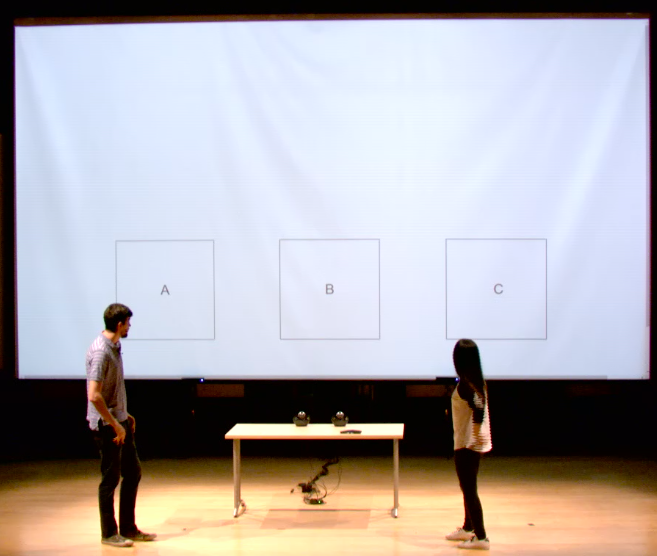
\includegraphics[width=0.7\columnwidth]{chapters/06_planning/figures/blockworld_demo_start.png}
  \caption{Starting state of our system.}
  \label{fig:blockworld_start}
\end{figure}

As a demonstration of our formalization process, we utilize our CAIS to solve the
false-belief task from before, modified to fit our CAIS. To accomplish this,
we instantiate a very elementary blocks world that involves only three blocks
named $\ablock$, $\bblock$, and $\cblock$, which all start on the
table. This is represented in the $\CEC$ as:

\begin{center}
\begin{tabular}{ c c }
    \holds(\on(\ablock, \ctable), 0) & 
    \holds(\clear(\ablock), 0)\\
    \holds(\on(\bblock, \ctable), 0) &     
    \holds(\clear(\bblock), 0)\\
    \holds(\on(\cblock, \ctable), 0) & 
    \holds(\clear(\cblock), 0)
\end{tabular}
\end{center}

In this instantiation, there are then two participants, \humana\ and \humanb\,
and then the block world is shown on the center screen in front of them. This
is shown in Figure~\ref{fig:blockworld_start}. We now provide below a sequence
of events that our agents act upon, providing the formalization of each action
into the \CEC\ as well as the fluent changes at each step of the time. If the
fluent is not removed by a step, then we assume that it carries over from the
previous step as is.

\begin{center}
\begin{tabular}{l | l | l}
    $t$ & Event in Natural Language & Event in \CEC\ \\
    \hline
    1 & \humana\ enters and registers with the CAIS & \happens(\register(\humana), 1) \\
    2 & \humanb\ enters and registers with the CAIS & \happens(\register(\humanb), 2) \\
    3 & \humana\ stacks block \ablock\ onto block \bblock\ & \happens(\stack(\ablock, \bblock), 3) \\
    4 & \humanb\ deregisters and leaves the CAIS & \happens(\deregister(\humanb), 4) \\
    5 & \humana\ unstacks block \ablock\ from block \bblock\ & \happens(\unstack(\ablock, \bblock), 5)
\end{tabular}\label{table:false_belief_actions}
\end{center}

\begin{center}
\begin{tabular}{l | l | l}
    $t$ & Added Fluent & Removed Fluents \\
    \hline
    1 & \holds(\inCAIS(\humana), 1) & \\
    2 & \holds(\inCAIS(\humanb), 2) & \\
    3 & \holds(\on(\ablock, \bblock)), 3) & \makecell[l]{
        \holds(\on(\ablock, \ctable), 2) \\
        \holds(\clear(\bblock), 2) \\
    }\\
    4 & & \holds(\inCAIS(\humanb), 3) \\
    5 & \makecell[l]{
        \holds(\on(\ablock, \ctable), 5) \\
        \holds(\clear(\bblock), 5) \\
    } & \makecell[l]{
        \holds(\on(\ablock, \bblock), 4) \\
    }
\end{tabular}\label{table:false_belief_fluents}
\end{center}

For this test, we utilize our weakest form of vicinity for agents, wherein
all events and fluents that happen within the room are in the vicinity of
any agent in the CAIS, and as such the agent can perceive them. If an agent
is outside the CAIS, then they are considered outside the vicinity of those
events and fluents, and will thus not perceive them. Additionally, for
any agents in the CAIS, they know, per our definition of $\textbf{I}_{1}^{f}$
that then all agents, being in the CAIS not only perceive the fluents for
themselves, but also that they perceive the other agents perceiving those
fluents as well. Additionally, we know from $\textbf{I}_{3}^{f}$ that our
CAIS also perceives all fluent changes, and perceives the agent perceiving
these fluents as well. From instantiations of $R_{1}$ - $R_{4}$ of the \CEC\
inference schemata, we can derive from these perceptions the state of beliefs
of our agents at any given time step to match the fluents that they perceive
at that time step.

\begin{figure}
  \begin{center}
    \begin{minipage}[b]{0.25\textwidth}
      \begin{flushleft}   
        \begin{footnotesize} \underline{\humana's beliefs}\\
          \vspace{4pt}
          \vspace{-4pt}
          \textbf{belief}:
        \end{footnotesize}
      \end{flushleft}    
      \begin{center} \begin{tikzpicture}[auto centering, background rectangle/.style={fill=white}, show background rectangle]
          \node[style=block] (C) {$C$};
          \node[style=empty] (E) [above=of C] {};
          \node[style=block] (B) [left=of C, left=.5cm of C] {$B$};
          \node[style=block] (A) [left=of B, left =.5 cm of B] {$A$};
        \end{tikzpicture}
      \end{center}
    \end{minipage}
   \hspace{50pt}
    \begin{minipage}[b]{0.25\textwidth}
      \begin{flushleft} 
        \begin{footnotesize} \underline{\humanb's  beliefs}\\                          
          \vspace{4pt}
          \vspace{-4pt}
          \textbf{belief}:
        \end{footnotesize}
      \end{flushleft}   \begin{tikzpicture}[auto centering, background rectangle/.style={fill=gray!25}, show background rectangle]
        \node[style=block] (B) {$B$};
        \node[style=emptyA] (E) [above=of C] {};
        \node[style=block] (A) [above=of B] {$A$};
        \node[style=block] (C) [right=of B, right=.5cm of B] {$C$};
        \node[style=empty] (F) [right=of C] {};
      \end{tikzpicture}
    \end{minipage}
  \end{center}
  \caption{Depiction of agents' mental states with the shaded portion indicating that \humanb\ is not in the room.}
  \label{fig:mom-example}
\end{figure}
 
We now move onto solving the false-belief task for our CAIS, and we consider
the world now after the completion of step 5. At this point, we wish to see
where the CAIS believes
the blocks are, as well as where it believes that \humana\ and
\humanb\ think the blocks are, focusing primarily on block A.  We ask
our overseeing AI three questions, translating them into the \CEC:

\begin{center}
\begin{tabular}{l|l}
    Where does the CAIS believe block \ablock\ is? & $\exists x (\believes(CAIS, 5, \holds(\on(\ablock, x), 5)))$ \\
    \makecell[l]{Where does the CAIS believe \\ \hspace{1cm}\humana believe block \ablock\ is?} & $\exists x (\believes(CAIS, 5, \believes(\humana, 5, \holds(\on(\ablock, x), 5))))$ \\
    \makecell[l]{Where does the CAIS believe \\ \hspace{1cm}\humanb believe block \ablock\ is?} & $\exists x (\believes(CAIS, 5, \believes(\humanb, 5, \holds(\on(\ablock, x), 5))))$
\end{tabular}
\end{center}

\noindent
For the first two questions, the CAIS and the \humana\ perceived all fluent
changes within the room, and so the answer should be the same, that block \ablock\ 
is on the table. For the third question, as \humanb\ has left our room, and thus
did not perceive the \unstack\ action, should still believe that the \ablock\
is on \bblock\. This state of affairs is captured in Figure~\ref{fig:mom-example}.
Through \textsf{ShadowProver}, we obtain an answer to the above question
of where each agent believes the block is: 

\begin{center}
\begin{tabular}{l}
     $\believes(CAIS, 5, \holds(\on(\ablock, \ctable), 5))$\\
     $\believes(CAIS, 5, \believes(\humana, 5, \holds(\on(\ablock, \ctable), 5)))$ \\
     $\believes(CAIS, 5, \believes(\humanb, 5, \holds(\on(\ablock, \bblock), 5)))$
\end{tabular}
\end{center}

From this, we have now shown that our CAIS possesses  ``theory of mind'', able to
track beliefs of both itself and contained agents, and moreover answer questions
about it. This provides a valuable baseline of ability to our system as we move
onto planning and plan recognition.